% TODO Maybe add a summary of what we'r going to speak in this chapter
\section[Overview of Epilepsy disease]{Pathophysiology and Treatment of Epilepsy}
Epilepsy is a disorder of the brain characterized by a lasting predisposition to generate spontaneous epileptic seizures, and has a numerous neurobiological, cognitive, and psychosocial consequences \cite{defEpilepsy}.
Epilepsy affects over 50 million people worldwide, making it one of the most common neurological diseases globally. Over 75\% of those with active epilepsy are untreated, mostly concentrated in low-income and middle-income countries. \cite{defeating_epilepsy}
  \subsection*{Epidemiology e Mortality}
  Epilepsy incidence is bimodally distributed with two peaks: the first in the pediatric population less than 5 years old, and the second in people over the age of 50 years. The incidence is higher in low-income countries than high-income countries, thanks a contribution of poor hygiene, poor basic sanitation and higher risk of infection \cite{THIJS2019689}.
  Regardless the geographical location, the prevalence of active epilepsy is usually between 4 and 12 per 1000, risk factor vary by age group \cite{Fiest296}.

  The risk of death for a person with epilepsy is increased compared with the risk for the general population. Mortality can be divided into deaths directly (eg, status epilepticus, injuries, SUDEP \cite{Langan211}) or indirectly (eg, suicide, drowning) attributable to epilepsy \cite{Devinsky779}. SUDEP (Sudden Unexpected Death in Epilepsy) is one of the main causes of epilepsy-related death.
  \subsubsection*{Causes}
  Epilepsy can have both genetic and acquired causes, with the interaction of these factors in many cases. Established acquired causes include serious brain trauma, stroke, tumours, and brain problems resulting from a previous infection.

  \subsection*{Definitions}
  \subsubsection*{Epilepsy}
  The given definition of Epilepsy is usually practically applied as having two unprovoked seizures occurring more than 24h apart. But the International League Against Epilepsy (ILAE) proposed that epilepsy be considered to be a disease of the brain by any of the following conditions: \cite{defEpilepsy}

  \begin{itemize}
    \item At least two unprovoked seizures occurring more than 24h apart;
    \item A single unprovoked seizure if recurrence risk is high (>60\% over the next 10 years);
    \item Diagnosis of an epilepsy syndrome.
  \end{itemize}
  \subsubsection*{Seizure}
  An epileptic seizure is the clinical manifestation of an abnormal, excessive, purposeless and synchronized electrical discharge in the neurons, that leads to brief episodes of involuntary movement that may involve a part of the body (partial) or the entire body (generalized) and are sometimes accompanied by loss of consciousness and control of bowel or bladder function. \cite{WHO}
  
  \subsection*{Classification}
  Classification is made at three levels: seizure type, epilepsy type, and epilepsy syndromes. \cite{classification}
  \subsubsection*{Seizure type}
  % Maybe add some images to well explain the things
  Seizures are first classified by onset as either focal, generalized or unknown.
  \begin{itemize}
    \item Focal Onset: Affects one part of the brain. Usually limited to a specific region in one area of the brain. Level of awareness subdivides focal seizure in those with retained awareness and impaired awareness. Retained awareness means that the person is aware of self and environment during the seizure, even if immobile. In addition, focal seizures are sub-grouped as those with motor and non-motor manifestation.
    \item Generalized Onset: Affects most or all of the brain. Typically congenital and occurs simultaneously in both hemispheres of the brain. They are almost always accompanied by impaired awareness. Generalized seizures are divided into motor and non-motor (absence) seizures.
    \item Unknown: It is the case in which the onset is missed or obscured. 
  \end{itemize}
  
  \subsubsection*{Epilepsy type}
  Epilepsy are divided in: focal, generalized, combined generalized and focal, and unknown. The category combined epilepsy is used for those presenting both seizure types.

  \subsection*{Pathophysiology}
  Epileptogenesis is the process of converting a non-epileptic brain into one capable of generating spontaneous recurrent seizures. A seizure can be conceptualized as occurring when there is a distortion of the normal balance between excitation and inhibition within a neural network \cite{pathophysiology}. 
  
  Epileptogenic networks are widely distributed for generalized epilepsies, involving thalamocortical structures bilaterally. For focal epilepsies, networks involve neuronal circuits in one hemisphere, commonly limbic or neocortical \cite{classification}.

  \subsection*{Treatment}
  For most of the people with epilepsy, antiseizure medications are the main treatment modality, but despite of many different medications, the current drugs are effective in only 60-70\% of individuals, this percentage decrease for people who lives in low-income countries \cite{DUNCAN2006}.

  Up to a third of all individuals with epilepsy are refractory to medical therapy \cite{SpencerHuh2008}. Drug-resistant epilepsy is assumed after the "failure of adequate trials of two tolerated, appropriately choses and used antiseizure drug schedules to achieve sustained seizure freedom" \cite{drug_resist}. In those cases alternative non-pharmacological treatments including surgery and neurostimulatory interventions should be considered.
  When surgery is not possible because of the presence of multifocal or generalized epilepsy or whenever the epileptogenic focus lies in eloquent cortex that cannot removed, neurostimulation techniques are palliative options \cite{Englot2013}.

  Three neurostimulation devices are approved for the treatment of drug resistant epilepsy \cite{kiriakopoulos_cascino_britton_2018}.
  \begin{itemize}
    \item VNS is approved for treatment of focal epilepsy when surgery is not possible or does not work.
    \item RNS is a device that can record seizure activity directly from the brain and delivers stimulation to stop seizures.
    \item DBS sends signals to the brain electrode to stop signals that trigger a seizure.
  \end{itemize}

\section{Vagus Nerve Stimulation}
Vagus Nerve Stimulation (VNS) is a treatment used for the management of medically intractable epilepsy to reduce seizure rates. Furthermore, it showed positive effects in multiple other medical conditions, including essential tremors gastroparesis \cite{KRAHL2004135}, chronic tinnitus, stroke, post-traumatic stress disorder \cite{HAYS2013275}, chronic pain, Parkinson's disease, eating disorders, multiple sclerosis, migraine and Alzheimer's disease \cite{BRONCEL202037, BeekwilderBeems2010}.

VNS consists of a device implanted in the upper left thoracic region with a helical electrode placed around the left cervical nerve, which delivers intermittent electrical impulses to activate the vagus nerve.

VNS was implanted first time in four epilepsy patients by Penry and Dean in 1988 \cite{Penry1990}. After several large clinical studies, it was approved for seizures by the European Community in 1994 and Food ad Drug Administration in 1997. Clinical trials demonstrate that 24 to 48 months after the implantation of the device, 60\% of patients were considered as responders and 8\% of implanted patients became seizure free \cite{Englot2016}. Responders to VNS will be defined as those who experience 50\% or greater reduction in seizure frequency after VNS \cite{IBRAHIM2017634}. Although VNS is used in clinical practice the exact mechanistic of its effect in modulating seizures remain poorly understood.

Side effects of VNS are generally limited to coughing and/or hoarseness of the voice, they can be controlled by changing the stimulation parameters. To avoid cardiac side effects, a cuff electrode in most cases is implanted on the left vagal nerve.

\begin{figure}[h]
  \centering
  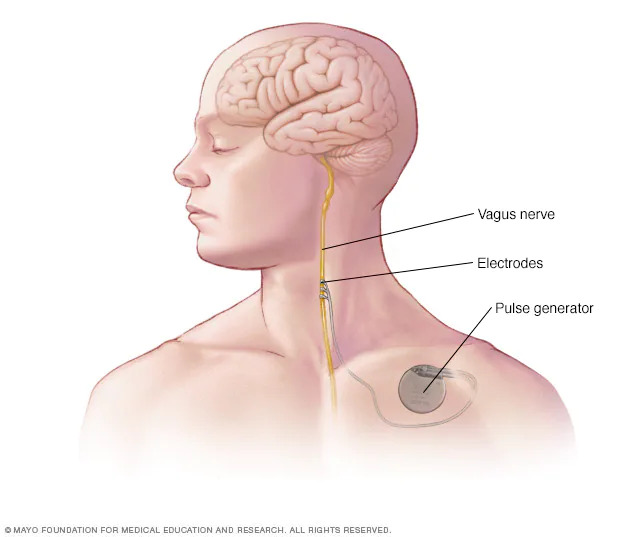
\includegraphics[width=0.8\textwidth]{images/vagus_nerve_stimulation.jpg}
  \caption{Components of the VS system.}
  \label{fig:Vagus Nerve Stimulation}
\end{figure}

  \subsection*{Vagus Nerve Anatomy and Connections}
  The vagal nerve (VN) is the longest cranial nerve and exerts a wide range of effects on the body. It comprises two nerves, the left and right vagus nerves and comprises both sensory and motor fibers.
  The vagal nerve is a mixed nerve made up of 75\% sensory(afferent) fibers responsible for coughing, swallowing, and voice sounds, and 25\% efferent fibers which mainly send feedback from hear, lungs, stomach and upper bowel.  \cite{BonazSinniger2017}.

  The majority of vagus nerve fibers are comprised of afferents and project to the nucleus tractus solitarius (NTS), which in turn sends fibers to other brainstem nuclei important in modulating the activity of subcortical and cortical circuitry (). This vagus afferent network (VagAN) is
  thought to be the neural substrate of VNS efficacy \cite{HanchemWongIbrahim2018}. 
  The NTS receives direct inputs from the VN and projects them to others brainstem nuclei: the locus coeruleus (LC), dorsal raphe nucleus (DRN), and parabranchial nucleus (PBN) \cite{RICARDO19781}. The functional importance of NTS connectivity in modulating seizure activity is further borne out by findings that increased inhibitory gamma-aminobutyric acid (GABA) signaling or decreased excitatory glutamate signaling within the NST reduces susceptibility to chemically induced limbic motor seizures \cite{GABA}.

  \begin{figure}[h]
    \begin{minipage}[c]{0.5\textwidth}
      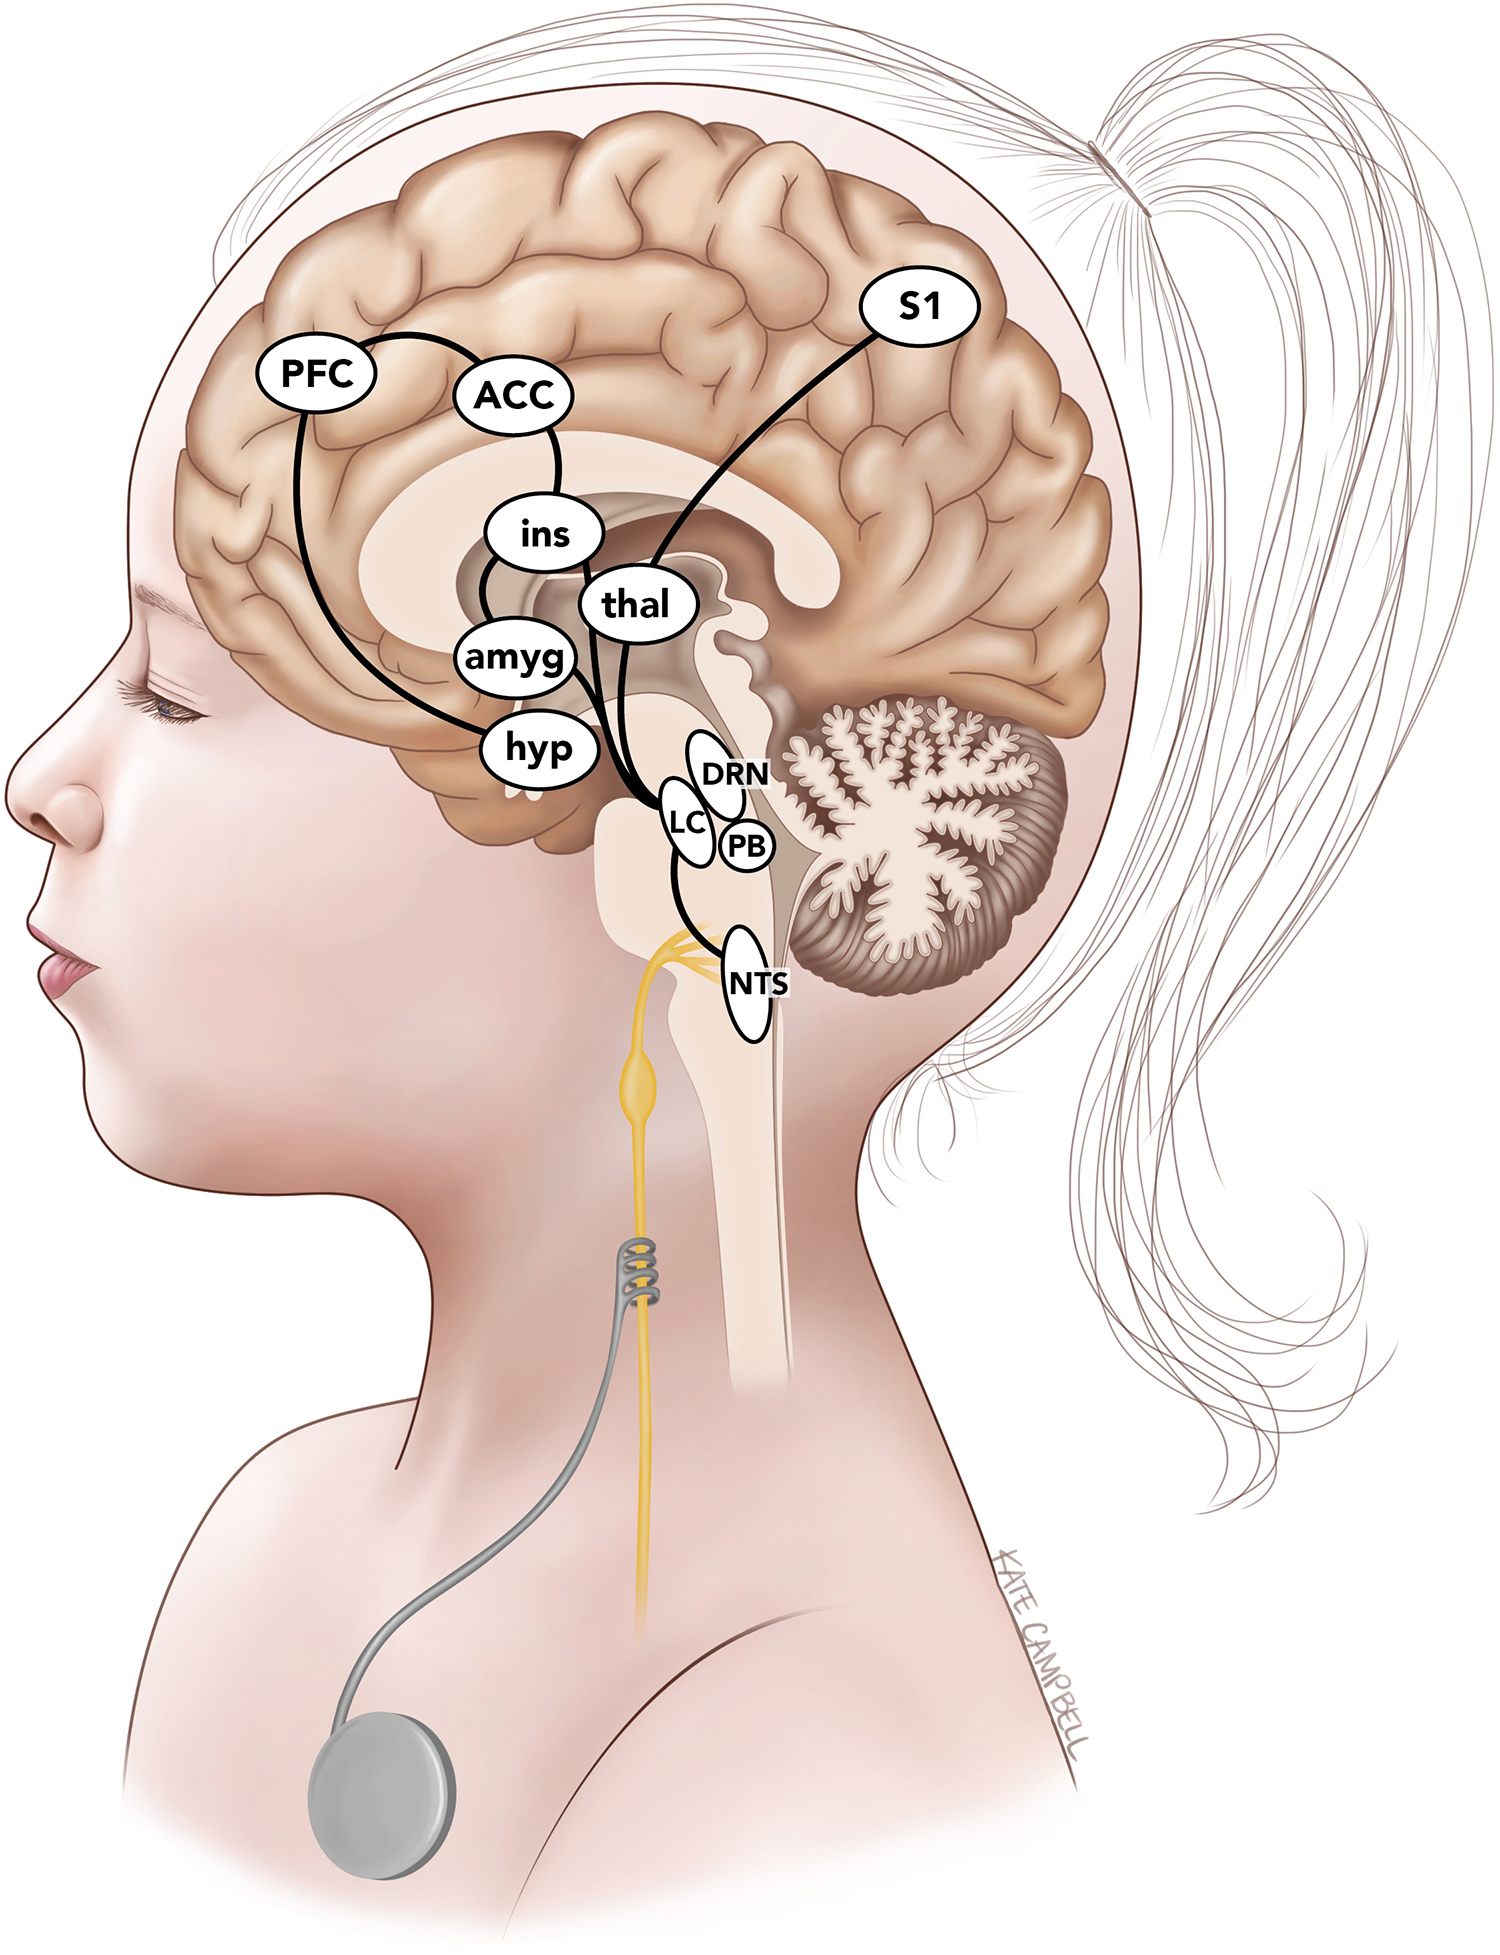
\includegraphics[width=\textwidth]{images/vagus_afferent_network.jpg}
    \end{minipage}\hfill
    \begin{minipage}[c]{0.5\textwidth}
      \caption{The vagus afferent network. Schematic diagram showing the important brainstem centers and subcortical and cortical structures. Copyright Kate Campbell, Medical \& Scientific Visualizations.} 
    \end{minipage}
    \centering
    \label{fig:Vagus Afferent Network}
  \end{figure}

  The LC is characterized by widely diffused projections to both subcortical and cortical structures. The projections of the LC are small unmyelinated fibers, forming a wide antero-posterior branching network to reach the raphe nuclei, the cerebellum, and almost all areas of the midbrain and forebrain regions. The LC is the main source of norepinephrine (NE) in the brain \cite{AGHAJANIAN1977570}. NE is a neurotransmitter that has been associated with the clinical effects of VNS by preventing seizure development and by inducing long-term plastic changes that could restore a normal function of the brain circuitry. Indeed, short bursts of VNS increase neuronal firing in the LC, leading to elevations in NE concentrations. \cite{BergerVespa2021}

  Studies have demonstrated indirect projection of the LC to the DRN, which sends widespread projections to upper cortical regions. DRN appears to have a more delayed response to VNS \cite{HanchemWongIbrahim2018}.

  Vagal afferents project to the PBN by way of both the NTS and LC. Cell bodies within the PBN send diffuse outputs to forebrain structures including the thalamus, insular cortex, amygdala, and hypothalamus. Moreover, PBN likely plays an important role in regulating thalamocortical circuitry that may be implicated in seizure generation. Specifically, PBN activates the intralaminar nuclei of the thalamus, which in turn relays sensory signals to widespread cortical areas. \cite{HanchemWongIbrahim2018}

  \subsection*{The Vagus Afferent Network}
  \subsubsection*{Thalamocortical Connections}
  Thalamocortical connections are believed to be an important substrate of VNS responsiveness because they modulate cortical excitability, rendering the brain less susceptible to seizures. The thalamus receives direct inputs from the NTS and PBN \cite{BecksteadJoel2980}. More recently, thalamic activation measured by BOLD fMRI was associated with improved VNS treatment response in patients with seizures \cite{NarayananWatts2002}. The importance of thalamocortical connections in mediating the VNS antiseizure effect is further borne out by findings that thalamic connections to the anterior cingulate and insular cortices are stronger in VNS responders \cite{IBRAHIM2017634}. % Qua questa citazione di Ibrahim è stata consiglita da Alex è utile per capire un pò il metodo.

  \subsubsection*{Limbic Circuitry}
  The limbic system is a collection of neuronal structures involved in controlling emotion, memory, behavior, and motivation. The fornix and stria terminalis showed more robust microarchitecture in VNS responders. The fornix is the main efferent tract of the hippocampus projecting to the mammillary bodies, nucleus accumbens, septal nuclei, anterior thalamic nuclei and cingulate cortex. While the stria terminalis forms the major input tract from the amygdala to the hypothalamus. 
  VNS has been shown to alter the structure and function of these regions, implicating the limbic system in its antiseizure action. \cite{Mithani2019}

\section{Literature of DW-MRI in VNS}
